\documentclass{article}
\usepackage{minted}
\usepackage{graphicx} % Required for inserting images
%-- coding: UTF-8 --
\usepackage[UTF8]{ctex}
\usepackage{amsmath}
\usepackage{xcolor} % to access the named colour LightGray
\definecolor{LightGray}{gray}{0.9}

%\newcommand{\subsubsubsection}[1]{\paragraph{#1}\mbox{}\\}
%\setcounter{secnumdepth}{4} % how many sectioning levels to assign numbers to
%\setcounter{tocdepth}{4} % how many sectioning levels to show in ToC


\title{数据结构期中大作业}
\author{软件工程1班 2106050130 徐圣翔}
\date{\today}

\begin{document}

\maketitle

\graphicspath{{picture/}}

\newpage
\tableofcontents
\newpage

\section{问题背景}
在计算机编程语言中,描述整数常用的数据类型有int、long long等,然而int所能表示的范围为$[-2147483648,+2147483647]$,long long所能表示的范围为$[-9223372036854775808,+9223372036854775807]$,最多只能表示19位的整数。当我们需要想要进行更大的整数运算时,内置数据类型已经不足以满足要求。

然而,大整数运算在现实世界中有着广泛的应用,例如在密码学、计算机图形学、数字信号处理和数值分析等领域。处理大整数的需求随着科技和计算能力的不断发展而日益增长,而传统的整数类型和算法在面对这些庞大的数字时往往力不从心。因此,研究和实现大整数运算的方法变得尤为重要。

\section{问题描述}
大整数运算问题涉及对非常大的整数执行各种算术和高级数学操作。这些整数的规模远远超过了计算机硬件和编程语言默认支持的整数范围,因此需要特殊的算法和数据结构来实现,通常包括以下几个方面:

\begin{enumerate}
    \item 整数表示:在计算机中,整数通常用二进制表示。然而,当涉及到大整数时,这些数可能具有数千甚至数百万位。为了有效地存储和操作这些大整数,需要使用特殊的数据结构,如链表、数组或其他自定义结构。
    \item 基本算术运算:大整数的加法、减法、乘法和除法等基本算术运算需要特殊的算法来实现。
    \item 高级数学操作:除了基本算术运算外,大整数运算还涉及高级数学操作,如求幂、开方、对数、因数分解、求最大公约数等。这些操作需要在有限的计算资源内高效地实现,往往需要巧妙的算法和优化策略。
    \item 性能和优化:大整数运算通常涉及大量的计算,因此算法性能至关重要。在设计大整数运算算法时,需要充分考虑计算效率、内存消耗和稳定性等因素。通过并行计算、分治策略和其他优化技巧,可以提高大整数运算的性能。
\end{enumerate}

总之,大整数运算问题描述了在计算机科学和数学领域如何处理和操作非常大的整数的挑战。我们需要开发高效的算法和数据结构,以应对各种应用场景中的大整数运算需求。

\section{模型分析}
在计算机科学领域,大整数运算是一个关键的问题。当数字超过计算机基本数据类型的表示范围时,就需要特殊的算法和数据结构来处理这些大整数。本文将对大整数运算的模型进行分析,主要探讨算法、数据结构以及优化策略。

一、数据结构

\begin{enumerate}
    \item 数组表示法:将大整数的每一位用数组的元素来表示,这种方法可以方便地扩展大整数的位数,适用于大整数的加法、减法、乘法等基本运算。
    \item 链表表示法:将大整数的每一位用链表的节点来表示,链表表示法有利于在运算过程中动态调整大整数的长度,适用于大整数的除法等复杂运算。
\end{enumerate}

二、算法

\begin{enumerate}
    \item 加法:采用逐位相加的方法,从低位到高位依次计算,需要注意进位的处理。时间复杂度为 O(max(m, n)),其中 m 和 n 分别是两个大整数的位数。
    \item 减法:类似于加法,采用逐位相减的方法,从低位到高位依次计算,需要注意借位的处理。时间复杂度为 O(max(m, n))。
    \item 乘法:可以采用传统的竖式乘法方法,时间复杂度为 O(m * n)。此外,还可以使用分治法如 Karatsuba 算法或快速傅里叶变换 (FFT) 等高效算法进行优化,降低时间复杂度。
    \item 除法:可以采用试商法或者牛顿迭代法进行大整数除法运算。试商法的时间复杂度为 O(m * n),牛顿迭代法可以降低时间复杂度。
\end{enumerate}

三、优化策略

\begin{enumerate}
    \item 通过减少数据结构中的冗余信息,可以提高大整数运算的性能。例如,在数组表示法中,可以用一个整数变量记录大整数的有效长度,从而避免处理大量的无效零位。
    \item 根据具体问题场景选择合适的算法。例如,在进行大整数乘法时,可以根据两个大整数的位数选择传统竖式乘法或者 FFT 等高效算法。
    \item 使用并行计算技术。针对多核处理器和 GPU 等并行计算设备,可以将大整数运算的一些子任务进行并行处理,以提高运算效率。
    \item 利用数学性质进行优化。例如,在进行大整数模运算时,可以利用模运算的分配律、结合律等性质,对大整数运算进行简化,从而提高运算效率。
\end{enumerate}

\section{算法设计}

由于正整数与负整数的运算以及负整数与负整数的运算都可以转换为正整数与正整数的运算,因此这里只考虑正整数与正整数的运算。

\subsection{进制转换}

题目要求先将大整数转为二进制,再把二进制中的每一位的0或1以字符$'0'$或$'1'$的形式从低到高依次存放在一个字符数组中,作为大整数的二进制字符表示。

通常情况下,十进制整数转为二进制通常采用模2取余的方法,二进制整数转为十进制整数通常采用加2的幂的方法,也就是说会,十进制转二进制会用到高精度除低精度,二进制转十进制会用到高精度加高精度,而转换为二进制的意义就是实现高精度大整数的加减乘除运算,所以此处不采用二进制表示法,而是直接采用十进制字符表示。


\subsection{整数表示}
在实现中,高精度数字利用字符串表示,每一个字符表示数字的一个十进制位。因此,高精度数值计算实际上是一种特别的字符串处理。

读入字符串时,数字最高位在字符串首(下标小的位置)。但是习惯上,下标最小的位置存放的是数字的最低位,即存储反转的字符串。这么做的原因在于,数字的长度可能发生变化,但我们希望同样权值位始终保持对齐(例如,希望所有的个位都在下标[0],所有的十位都在下标[1]......);同时,加、减、乘的运算一般都从个位开始进行,因此我们采用反转存储的字符数组来表示整数。

代码如下:

\begin{minted}
[
frame=lines,
framesep=2mm,
baselinestretch=1.2,
bgcolor=LightGray,
fontsize=\footnotesize,
linenos
]
{c}
#include <stdio.h>

const int N = 100010;

char a[N], b[N];                // 存储待运算数字
int lena, lenb;

int A[N], B[N], C[N];           // C用于存储答案
int lenA, lenB, lenC;

int get_lenth(char s[]);

int main()
{
    scanf(" %s %s", a, b);      // 过滤空格与换行符
    
    lena = get_lenth(a), lenb = get_lenth(b);

    for(int i = lena - 1; i >= 0; i --) A[lenA ++] = (a[i] - '0');      // 倒序存储
    for(int j = lenb - 1; j >= 0; j --) B[lenB ++] = (b[j] - '0');

    printf("a = %s\nlength of a = %d\nb = %s\nlength of b = %d\n", a, lena, b, lenb);
    printf("A:\n");
    for(int i = 0; i < lenA; i ++)  printf("%d", A[i]);
    printf("\nB:\n");
    for(int i = 0; i < lenB; i ++)  printf("%d", B[i]);
    return 0;
}

int get_lenth(char s[])
{
    int len = 0;
    for(int i = 0; s[i] != '\0'; i ++)  len ++;
    return len;
}
\end{minted}

当输入为"132456123"和"951357"两个字符数组时,输出为
\begin{minted}
[
frame=lines,
framesep=2mm,
baselinestretch=1.2,
bgcolor=LightGray,
fontsize=\footnotesize,
linenos
]
{c}
a = 123456123
length of a = 9
b = 951357
length of b = 6
A:
321654321
B:
753159
\end{minted}

不难看出,我们将字符数组倒转并存进了整数数组内,并保持了权值位对齐。

\subsection{高精度加法}
高精度加法,本质上是对竖式加法进行模拟。

\begin{figure}[htp]
    \centering
    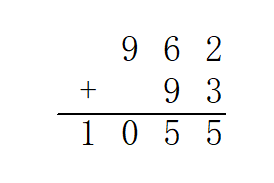
\includegraphics[width=4cm]{picture/Additive vertical.png}
    \caption{竖式加法}
\end{figure}

从最低位开始,将两个加数对应位置上的数码相加,并判断是否达到或超过10。如果达到,那么处理进位:将更高一位的结果上增加1,当前位的结果减少10。

针对进位我们可以使用一个变量来存储是否进位,若变量为1,在后一位的计算中便要加1,否则加0。

同时,在竖式加法中,我们更倾向于用较大位数的数做加数,较小位数的数做减数,因此,我们需要根据长度决定是否要交换两个操作数。

代码如下(仅展示核心代码):

\begin{minted}
[
frame=lines,
framesep=2mm,
baselinestretch=1.2,
bgcolor=LightGray,
fontsize=\footnotesize,
linenos
]
{c}
int max(int a, int b);          // 求较大值
void swap(int* a, int* b);      // 交换数值
void add(int *A, int *B);       // 加法

int main()                      
{
    if(lenA < lenB)             // 如果A的位数比B少,那么交换A和B的值
    {
        for(int i = 0; i < max(lenA, lenB); i ++)
            swap(&A[i], &B[i]);
        swap(&lenA, &lenB);
    }

    add(A, B);
    for(int i = lenC - 1; i >= 0; i --) printf("%d",C[i]);      // 倒序输出答案数组

    return 0;
}

int max(int a, int b)
{
    return (a > b) ? a : b;
}

void swap(int* a, int* b)           // 交换a与b的值
{
    *a = *a ^ *b;
    *b = *a ^ *b;
    *a = *a ^ *b;
}

void add(int *A, int *B)
{
    int t = 0;              // 存储进位信息
    for (int i = 0; i < lenA; i ++ )
    {
        t += A[i];
        if (i < lenB) t += B[i];
        C[lenC ++] = t % 10;        // 处理进位信息
        t /= 10;
    }

    if (t) C[lenC ++] = t;          // 处理最高位的进位
    return ;
}
\end{minted}

\subsection{高精度减法}
同理,高精度减法也是模拟竖式减法的过程。

\begin{figure}[htp]
    \centering
    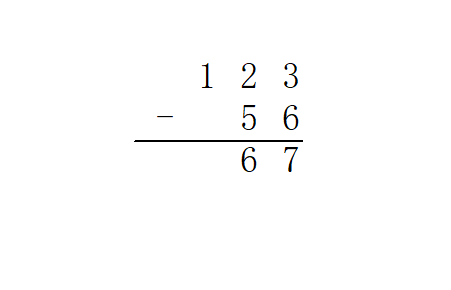
\includegraphics[width=4cm]{picture/Subtraction vertical.png}
    \caption{竖式减法}
\end{figure}

先判断两个数的大小,如果减数小于被减数,将其转化为-(被减数-减数)。从个位起逐位相减,遇到负的情况则向上一位借1。整体思路与加法完全一致。

代码如下(仅展示核心代码):

\begin{minted}
[
frame=lines,
framesep=2mm,
baselinestretch=1.2,
bgcolor=LightGray,
fontsize=\footnotesize,
linenos
]
{c}
int cmp(int A[], int B[]);      // 比较待运算数字大小
int max(int a, int b);          // 求较大值
void swap(int* a, int* b);      // 交换数值
void sub(int *A, int *B);       // 减法

int main()
{
    if(!cmp(A, B))              // 如果A比B小,那么转变成-(B-A)
    {
        printf("-");
        for(int i = 0; i < max(lenA, lenB); i ++)
            swap(&A[i], &B[i]);
        swap(&lenA, &lenB);
    }
    sub(A, B);
    for(int i = lenC - 1; i >= 0; i --) printf("%d",C[i]);

    return 0;
}

int cmp(int A[], int B[])
{
    // 如果A的位数比B小,那么A<B;
    // 如果A的位数和B相同,那么从高位到低位依次比较大小
    if(lenA != lenB)    return ((lenA > lenB) ? 1 : 0);
    for(int i = lenA - 1; i >= 0; i --)
    {
        if(A[i] != B[i])    return ((A[i] > B[i]) ? 1 : 0);
    }
    return 1;
}

int max(int a, int b)
{
    return (a > b) ? a : b;
}

void swap(int* a, int* b)
{
    *a = *a ^ *b;
    *b = *a ^ *b;
    *a = *a ^ *b;
}

void sub(int *A, int *B)
{
    int t = 0;
    for (int i = 0; i < lenA; i ++)
    {   
        t = A[i] - t;                       // 处理进位
        if(i < lenB) t -= B[i];             // 对位进行计算
        C[lenC ++] = (t + 10) % 10;         // 计算本位的数
        if(t < 0)   t = 1;                  // 确定是否进位
        else    t = 0;
    }

    while (lenC > 1 && C[lenC - 1] == 0) lenC --;       // 去除前导0
    return ;
}
\end{minted}

\subsection{高精度乘法}
在计算高精度与高精度的乘法之前,我们先介绍高精度与低精度的乘法。

\subsubsection{高精度乘低精度}
高精度乘低精度,即有一个乘数处于int范围内。对于这种情况,在竖式乘法中,我们通常将乘数整体与被乘数的每一位相乘,然后相加。

\begin{figure}[htp]
    \centering
    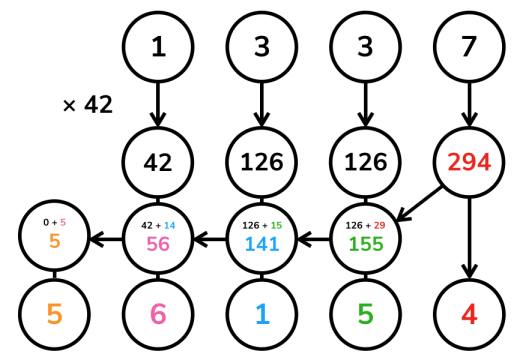
\includegraphics[width=4cm]{picture/Multiplication vertical.png}
    \caption{竖式乘法}
\end{figure}

以$1337 \times 42$为例,$7\times 42 = 294$,将4留在个位,29参与到下一位的运算中,$3\times 42 + 29 = 126$,在十位留6,12继续参与下一位的运算,直至最高位运算完成,得到"45165",倒序输出得到答案56154.

总结一下,对于第i位,上$A_i\times b \% 10$,进$A_i\times b / 10$。那么也就存在这样一种情况,到最后可能已经运算结束,但是存储进位的变量里还存着首位的1,所以在最后判断进位变量是否存储值。

代码如下(仅展示核心代码):

\begin{minted}
[
frame=lines,
framesep=2mm,
baselinestretch=1.2,
bgcolor=LightGray,
fontsize=\footnotesize,
linenos
]
{c}
void mul(int A[], int b);       // 乘法

int main()
{
    mul(A, b);
    for(int i = lenC - 1; i >= 0; i --) printf("%d",C[i]);

    return 0;
}

void mul(int A[], int b)
{
    int t = 0;
    for (int i = 0; i < lenA || t; i ++ )
    {
        if (i < lenA) t += A[i] * b;
        C[lenC ++] = t % 10;                // 留下个位
        t /= 10;                            // 进位信息
    }

    while (lenC > 1 && C[lenC - 1] == 0) lenC --;       // 去除前导0
    return ;
}
\end{minted}

\subsubsection{高精度乘高精度}

那么,已经解决了高精度乘低精度,在来考虑高精度乘高精度便容易许多了。再来重复竖式乘法的过程:

\begin{figure}[htp]
    \centering
    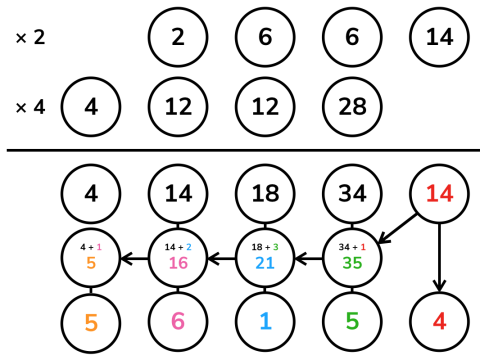
\includegraphics[width=4cm]{picture/Multiplication-long vertical.png}
    \caption{高精度竖式乘法}
\end{figure}

实际上是计算了若干$a\times b_i \times 10^i $的和。例如,当我们计算$1337\times 42$时,计算的是$1337 \times 2 \times 10^0 + 1337 \times 4 \times 10^1$。

于是可以将被乘数分解为它的所有数码,其中每个数码都是低精度数,将它们分别与乘数相乘,再向左移动到各自的位置上相加即得答案。当然,最后也需要用与以上高精度与低精度相乘运算相同的方式处理进位。

注意这个过程与传统的竖式乘法不尽相同,我们的算法在每一步乘的过程中并不进位,而是将所有的结果保留在对应的位置上,到最后再统一处理进位,但这不会影响结果。

也可以计算结果中的从低到高第i位,且一并处理进位。第i次循环为$c[i]$加上了所有满足$p+q=i$的$a[p]$与$b[q]$的乘积之和,这样做的效果和直接进行上图的运算最后求和是一样的,只是更加简短的一种实现方式。

与加法类似的,我们也更习惯于用位数较长的数乘位数较少的数,因此会在计算之前加以判断。

代码如下(仅展示核心代码):

\begin{minted}
[
frame=lines,
framesep=2mm,
baselinestretch=1.2,
bgcolor=LightGray,
fontsize=\footnotesize,
linenos
]
{c}
int max(int a, int b);          // 求较大值
void swap(int* a, int* b);      // 交换数值
void mul(int *A, int *B);       // 乘法

int main()
{
    if(lenA < lenB)
    {
        for(int i = 0; i < max(lenA, lenB); i ++)
            swap(&A[i], &B[i]);
        swap(&lenA, &lenB);
    }

    mul(A, B);
    for(int i = lenC - 1; i >= 0; i --) printf("%d",C[i]);

    return 0;
}

int max(int a, int b)
{
    return (a > b) ? a : b;
}

void swap(int* a, int* b)
{
    *a = *a ^ *b;
    *b = *a ^ *b;
    *a = *a ^ *b;
}

void mul(int *A, int *B)
{
    // 两个数相乘,结果的位数不会多于两数位数之和+1
    for (int i = 0; i < lenA + lenB + 1; ++i) 
    {
        for (int j = 0; j <= i; ++j)
            C[i] += A[j] * B[i - j];        // 加上所有满足p+q=i的元素的乘积之和
        if(C[i] >= 10)
        {
            C[i + 1] += C[i] / 10;
            C[i] %= 10;
        }
        lenC ++;
    }

    while (lenC > 1 && C[lenC - 1] == 0) lenC --;       // 去除前导0
    return ;
}
\end{minted}

\subsubsection{高精度乘法与多项式乘法}
如果数据规模达到了$10^{10^5}$或更大,普通的高精度乘法可能会耗时过久,因此这里引入多项式乘法来优化高精度乘法。

一般多项式表示为:$f(x)=a_nx^n+a_{n-1}x^{n-1}+...+a_0$。

对于一个n位的十进制整数a,可以将它看作一个每位系数均为整数且不超过$10$的多项式 $A=a_{0} 10^0+a_{1} 10^1+\cdots+a_{n-1} 10^{n-1}$。这样,我们就将两个整数乘法转化为了两个多项式之间的乘法。

\subsubsection{快速傅里叶变换}
首先,我们先介绍多项式的表示形式,即系数表示与点值表示,$f(x)$的系数表示为$f(x)=a_nx^n+a_{n-1}x^{n-1}+...+a_0$。$f(x)$的点值表示为$(x_0,f(x_0)),(x_1,f(x_1)),...,(x_n,f(x_n))$。

不难发现,$n+1$个点值可以表示一个$n$次多项式,且在点值表示下,$n$次多项式的乘法复杂度为$O(n)$。$h(x)=f(x)g(x)$ $h(x)$为$n$次多项式,对于同一$x_i$,$h(x_i)=f(x_i)g(x_i)$。对于$f(x)*g(x)$函数,先将$f(x)$和$g(x)$转为点值表示,再利用$O(n)$的乘法得到$h(x)$的点值表示再转化为系数表示。

接下来,我们介绍复数与单位根的概念。复数可以用指数形式表示为:$a+bi=re^{i\theta}$,其中$r=\sqrt{a^2+b^2},tan(\theta)=\frac{b}{a}$。$x^n=1$在复数域上的根称为n次单位根。

$n$次单位根有$n$个,形式为$\omega_n^k=e^{i\frac{2k\pi}{n}}$。单位根具有如下性质:
\begin{equation*}
    \omega_n^k=\omega_{2n}^{2k}
\end{equation*}
\begin{equation*}
    \omega_{2n}^{k+n}=-\omega_{2n}^k
\end{equation*}

对于傅里叶变换在信号领域的原理与应用我们不做过多阐述。

离散傅里叶变换(DFT,Discrete Fourier Transform),可以将多项式$A(n)=a_0+a_1x+...+a_{n-1}x^{n-1}$转化为点值形式$(\omega_n^k,A(\omega_n^k)),\;(k=0,1,...,n-1)$。

逆离散傅里叶变换(IDFT,Inverse Discrete Fourier Transform),可以将多项式$(\omega_n^k,A(\omega_n^k)),\;(k=0,1,...,n-1)$转化为点值形式$A(n)=a_0+a_1x+...+a_{n-1}x^{n-1}$。

FFT 算法的基本思想是分治。就DFT来说,它分治地来求当 
$x=\omega_n^k$的时候$f(x)$的值。FFT的分治思想体现在将多项式分为奇次项和偶次项处理。

不妨令令$n=2^l$,有
\begin{equation*}
    A(n)=(a_0+a_2x^2+...+a_{n-2}x^{n-2}) + (a_1x+a_3x^3+...+a_{n-1}x^{n-1})
\end{equation*}
\begin{equation*}
    B(x)=a_0+a_2x+...+a_{n-2}x^{\frac{n}{2}-1}
\end{equation*}
\begin{equation*}
    C(x)=a_1+a_3x+...+a_{n-1}x^{\frac{n}{2}-1}
\end{equation*}

那么,便有$A(x)=B(x^2)+x \times C(x^2)$。利用偶数次单位根的性质$\omega^i_n = -\omega^{i + n/2}_n$,和 $B\left(x^2\right)$ 和 $C\left(x^2\right)$是偶函数,我们知道在复平面上$\omega^i_n$和$\omega^{i+n/2}_n $的 $B(x^2)$ 和 $C(x^2)$ 对应的值相同。得到:

得到:

\begin{equation*}
\begin{split}
A(\omega_n^k) &= B((\omega_n^k)^2) + \omega_n^k  \times C((\omega_n^k)^2) \\ 
              &= B(\omega_n^{2k}) + \omega_n^k  \times C(\omega_n^{2k}) \\
              &= B(\omega_{n/2}^k) + \omega_n^k  \times C(\omega_{n/2}^k) \\
\end{split}
\end{equation*}

和: 
\begin{equation*}
\begin{split}
A(\omega_n^{k+n/2}) &= B(\omega_n^{2k+n}) + \omega_n^{k+n/2}                        \times C(\omega_n^{2k+n}) \\
                    &= B(\omega_n^{2k}) - \omega_n^k  \times C(\omega_n^{2k}) \\
                    &= B(\omega_{n/2}^k) - \omega_n^k  \times C(\omega_{n/2}^k) \\
\end{split}
\end{equation*}

因此我们求出了$B(\omega_{n/2}^k)$和$C(\omega_{n/2}^k)$后,就可以同时求出$A(\omega_n^k)$和$A(\omega_n^{k+n/2})$。于是对$B$和$C$分别递归 DFT即可。

考虑到分治$DFT$能处理的多项式长度只能是$2^m(m \in \mathbf{N}^ \ast )$,否则在分治的时候左右不一样长,右边就取不到系数了。所以要在第一次$DFT$之前就把序列向上补成长度为 $2^m(m \in \mathbf{N}^\ast )$(高次系数补 0)、最高项次数为 $2^m-1$ 的多项式。

在代入值的时候,代入 
$\omega_n^0$,$\omega_n^1$,$\omega_n^2$,$\cdots$, $\omega_n^{n-1}$ $(n=2^m(m \in \mathbf{N}^ \ast ))$ 一共 $2^m$ 个不同值。因为是单位复根,所以说我们需要令 n 项式的高位补为零,使得 $n = 2 ^ k, k \in \mathbf{N}^ \ast$。

为方便理解,我们举一个8项多项式的例子:
$f(x) = a_0 + a_1x + a_2x^2+a_3x^3+a_4x^4+a_5x^5+a_6x^6+a_7x^7$
按照次数的奇偶来分成两组,然后右边提出来一个$x$:
\begin{equation*}
    \begin{split}
        f(x) &= (a_0+a_2x^2+a_4x^4+a_6x^6) + (a_1x+a_3x^3+a_5x^5+a_7x^7)\\
             &= (a_0+a_2x^2+a_4x^4+a_6x^6) + x(a_1+a_3x^2+a_5x^4+a_7x^6)
    \end{split}
\end{equation*}

分别用奇偶次次项数建立新的函数:
\begin{equation*}
    \begin{split}
        G(x) &= a_0+a_2x+a_4x^2+a_6x^3\\
        H(x) &= a_1+a_3x+a_5x^2+a_7x^3
    \end{split}
\end{equation*}

那么原来的 f(x) 用新函数表示为:
$f(x)=G\left(x^2\right) + x  \times  H\left(x^2\right)$

当然,这个算法还可以继续优化。对于$FFT$,我们每一次都会把整个多项式的奇数次项和偶数次项系数分开,一直分到只剩下一个系数。但是,这个递归的过程需要更多的内存。因此,我们可以先模仿递归过程,把这些系数在原数组中拆分,然后再倍增地去合并这些算出来的值。

对于\textbf{拆分},可以使用位逆序置换实现。

对于\textbf{合并},使用蝶形运算优化可以做到只用$O(1)$的额外空间来完成。

对于位逆序置换,我们不妨先举例予以说明:
\begin{itemize}
    \item 初始序列为${x_0,x_1,x_2,x_3,x_4,x_5,x_6,x_7}$
    \item 第一次置换${x_0,x_2,x_4,x_6},{x_1,x_3,x_5,x_7}$
    \item 第二次置换${x_0,x_4},{x_2,x_6},{x_1,x_5},{x_3,x_7}$
    \item 第三次置换${x_0},{x_4},{x_2},{x_6},{x_1},{x_5},{x_3},{x_7}$
\end{itemize}

也许这样还不够明显,那我们不妨转为二进制来观察规律:
\begin{itemize}
    \item 初始序列为${000,001,010,011,100,101,110,111}$
    \item 置换序列为${000,100,010,110,001,101,011,111}$
\end{itemize}

不难发现,置换序列本质上是将初始序列的下标转为二进制表示并逆序翻转,将翻转后得到的结果作为置换序列的下标。

实际上,位逆序置换可以从小到大递推实现,设$len=2^k$,其中$k$表示二进制数的长度,设$R(x)$表示长度为$k$的二进制数$x$翻转后的数(高位补0)。我们要求的是 $R(0),R(1),\cdots,R(n-1)$。

首先$R(0)=0$,从小到大求$R(x)$。因此在求$R(x)$时,
$R\left(\left\lfloor \dfrac{x}{2} \right\rfloor\right)$ 的值是已知的。因此我们把$x$右移一位,然后翻转,再右移一位,就得到了 $x$ 除了(二进制)个位之外其它位的翻转结果。考虑个位的翻转结果:如果个位是 $0$,翻转之后最高位就是 $0$。如果个位是 $1$,则翻转后最高位是 $1$,因此还要加上
$\dfrac{len}{2}=2^{k-1}$。综上:

\begin{equation*}
    \begin{split}
        R(x)=\left\lfloor \frac{R\left(\left\lfloor \frac{x}{2} \right\rfloor\right)}{2} \right\rfloor + (x\bmod 2)\times \frac{len}{2}
    \end{split}
\end{equation*}

已知 
$B(\omega_{n/2}^k)$和$C(\omega_{n/2}^k)$后,需要使用下面两个式子求出$A(\omega_n^k)$和$A(\omega_n^{k+n/2})$:

\begin{equation*}
    \begin{split}
    A(\omega_n^k)       & = B(\omega_{n/2}^k) + \omega_n^k \times C(\omega_{n/2}^k) \\
    A(\omega_n^{k+n/2}) & = B(\omega_{n/2}^k) - \omega_n^k \times C(\omega_{n/2}^k)
    \end{split}
\end{equation*}

使用位逆序置换后,对于给定的 $n$, $k$:$B(\omega_{n/2}^k)$ 的值存储在数组下标为 $k$ 的位置,$C(\omega_{n/2}^k)$ 的值存储在数组下标为$k + \dfrac{n}{2}$ 的位置。$f(\omega_n^k)$ 的值将存储在数组下标为 $k$ 的位置,$f(\omega_n^{k+n/2})$ 的值将存储在数组下标为$k + \dfrac{n}{2}$ 的位置。因此可以直接在数组下标为 $k$ 和 $k + \frac{n}{2}$ 的位置进行覆写,而不用开额外的数组保存值。此方法即称为蝶形运算。

再详细说明一下如何借助蝶形运算完成所有段长度为$\frac{n}{2}$ 的合并操作:令段长度为$s = \frac{n}{2}$;同时枚举序列$\{B(\omega_{n/2}^k)\}$ 的左端点 $l_g = 0, 2s, 4s, \cdots, N-2s$ 和序列$\{C(\omega_{n/2}^k)\}$ 的左端点 $l_h = s, 3s, 5s, \cdots, N-s$;合并两个段时,枚举 $k = 0, 1, 2, \cdots, s-1$,此时$B(\omega_{n/2}^k)$ 存储在数组下标为 $l_g + k$ 的位置,$C(\omega_{n/2}^k)$ 存储在数组下标为 $l_h + k$ 的位置;使用蝶形运算求出$A(\omega_n^k)$ 和 $A(\omega_n^{k+n/2})$,然后直接在原位置覆写。

那么如何将得到的多项式点值表示$(\omega_n^k,A(\omega_n^k)),\;(k=0,1,...,n-1)$转化为点值形式$A(n)=a_0+a_1x+...+a_{n-1}x^{n-1}$呢?

不妨设$n\times n$的矩阵$\Omega$,其中$\Omega_{i,j}=\omega_{n}^{ij}$,设向量$a=(a_0,a_1,...,a_{n-1}),b=(b_0,b_1,...,b_{n-1})$,则IDFT相当于求解方程$\Omega a=b$,令$\overline{\Omega_{i,j}}=\omega_n^{-ij}$,因此$a=\frac{1}{n}\overline{\Omega}b$。相当于对于给定的$B(x)=b_0+b_1x+...+b_{n-1}x^{n-1}$,求点值$B(\omega_n^{-k}),\;(0 \leq k < n)$。

由于使用了一些C++特性,便采用C++描述,代码如下:

\begin{minted}
[
frame=lines,
framesep=2mm,
baselinestretch=1.2,
bgcolor=LightGray,
fontsize=\footnotesize,
linenos
]
{c}
#include <bits/stdc++.h>

using namespace std;

const double PI = acos(-1.0);
const int N = 200020;

struct Complex
{
    double x, y;

    Complex(double _x = 0.0, double _y = 0.0) 
    {
        x = _x;
        y = _y;
    }

    Complex operator - (const Complex &b) const 
    {
        return Complex(x - b.x, y - b.y);
    }

    Complex operator + (const Complex &b) const 
    {
        return Complex(x + b.x, y + b.y);
    }

    Complex operator * (const Complex &b) const 
    {
        return Complex(x * b.x - y * b.y, x * b.y + y * b.x);
    }
};

Complex x1[N], x2[N];
char str1[N / 2], str2[N / 2];
int sum[N];

void change(Complex y[], int len);      // 位逆序置换
void fft(Complex y[], int len, int on);

int main() 
{
    while(scanf("%s%s", str1, str2) == 2)
    {
        int len1 = strlen(str1);
        int len2 = strlen(str2);
        int len = 1;

        while (len < len1 * 2 || len < len2 * 2) len <<= 1;

        for (int i = 0; i < len1; i++) x1[i] = Complex(str1[len1 - 1 - i] - '0', 0);

        for (int i = len1; i < len; i++) x1[i] = Complex(0, 0);

        for (int i = 0; i < len2; i++) x2[i] = Complex(str2[len2 - 1 - i] - '0', 0);

        for (int i = len2; i < len; i++) x2[i] = Complex(0, 0);

        fft(x1, len, 1);
        fft(x2, len, 1);

        for (int i = 0; i < len; i++) x1[i] = x1[i] * x2[i];

        fft(x1, len, -1);

        for (int i = 0; i < len; i++) sum[i] = int(x1[i].x + 0.5);

        for (int i = 0; i < len; i++)
        {
            sum[i + 1] += sum[i] / 10;
            sum[i] %= 10;
        }

        len = len1 + len2 - 1;

        while (sum[len] == 0 && len > 0) len--;

        for (int i = len; i >= 0; i--) printf("%c", sum[i] + '0');

        printf("\n");
    }

    return 0;
}

void change(Complex y[], int len)
{
    int i, j, k;

    for (int i = 1, j = len / 2; i < len - 1; i++) 
    {
        if (i < j) swap(y[i], y[j]);

        k = len / 2;

        while (j >= k)
        {
            j = j - k;
            k = k / 2;
        }

        if (j < k) j += k;
    }
}

void fft(Complex y[], int len, int on)
{
    change(y, len);

    for (int h = 2; h <= len; h <<= 1)
    {
        Complex wn(cos(2 * PI / h), sin(on * 2 * PI / h));

        for (int j = 0; j < len; j += h) 
        {
            Complex w(1, 0);

            for (int k = j; k < j + h / 2; k++)
            {
                Complex u = y[k];
                Complex t = w * y[k + h / 2];
                y[k] = u + t;
                y[k + h / 2] = u - t;
                w = w * wn;
            }
        }
    }

    if (on == -1)
    {
        for (int i = 0; i < len; i++)
        {
            y[i].x /= len;
        }
    }
}
\end{minted}

\subsubsection{快速数论变换}

在快速傅里叶变换的基础上,我们还可以从数论的角度做进一步优化。
假设质数$p$满足$p=r2^l+1$,$g$是$p$的原根。那么使用$g_n=g^{\frac{p-1}{n}}$替代$\omega_n$,仍然满足如下性质:

\begin{equation*}
    \begin{split}
        g_{2n}^{2k} \equiv g_n^k(mod\;p),(2n\leq2^l) \\
        g_{2n}^n \equiv -1(mod\;p),(2n\leq2^l) \\
    \end{split}
\end{equation*}

\begin{equation*}
    \begin{split}
        \Sigma_{k=0}^{n-1}g_n^{ik}g_n^{-kj}=
        \begin{cases}
        n,\;if\quad i=j \\
        0,\;otherwise
        \end{cases}
        \quad (mod\;p)\quad 其中0\leq i,j<n
    \end{split}
\end{equation*}

便可以使用$g_n$替换FFT中的$\omega_n$,其余推导过程仍然成立,此处便不做赘述。NTT相较于FFT的优点在于更快更精确,避免了浮点精度误差,但是NTT中质模数需要满足$p=r2^l+1$。

代码如下:

\begin{minted}
[
frame=lines,
framesep=2mm,
baselinestretch=1.2,
bgcolor=LightGray,
fontsize=\footnotesize,
linenos
]
{c}
#include <bits/stdc++.h>

using namespace std;

const int N = 300100, P = 998244353;

int r[N];
int A[N], B[N], C[N];
char a[N], b[N];

int qpow(int x, int y);
void ntt(int *x, int lim, int opt);

int main()
{
    int i, lim = 1, n;
    scanf(" %s", &a);
    n = strlen(a);
    for (i = 0; i < n; ++i) A[i] = a[n - i - 1] - '0';
    while (lim < (n << 1)) lim <<= 1;

    scanf(" %s", &b);
    n = strlen(b);
    for (i = 0; i < n; ++i) B[i] = b[n - i - 1] - '0';
    while (lim < (n << 1)) lim <<= 1;

    for (i = 0; i < lim; ++i) r[i] = (i & 1) * (lim >> 1) + (r[i >> 1] >> 1);
    ntt(A, lim, 1);
    ntt(B, lim, 1);
    for (i = 0; i < lim; ++i) C[i] = 1ll * A[i] * B[i] % P;
    ntt(C, lim, -1);
    int len(0);
    for (i = 0; i < lim; ++i) 
    {
        if (C[i] >= 10)
        {
            len = i + 1;
            C[i + 1] += C[i] / 10;
            C[i] %= 10;
        } 
        if (C[i]) len = max(len, i);
    }
    while (C[len] >= 10)
    {
        C[len + 1] += C[len] / 10;
        C[len] %= 10;
        len++;
    }
    for (i = len; ~i; -- i) putchar(C[i] + '0');
    cout << endl;
    system("pause");
    return 0;
}

int qpow(int x, int y)
{
    int res = 1;
    while (y)
    {
        if (y & 1) res = 1ll * res * x % P;
        x = 1ll * x * x % P;
        y >>= 1;
    }
    return res;
}

void ntt(int *x, int lim, int opt)
{
    int i, j, k, m, gn, g, tmp;
    for (i = 0; i < lim; ++i)
        if (r[i] < i)   swap(x[i], x[r[i]]);
    for (m = 2; m <= lim; m <<= 1) 
    {
        k = m >> 1;
        gn = qpow(3, (P - 1) / m);
        for (i = 0; i < lim; i += m)
        {
            g = 1;
            for (j = 0; j < k; ++j, g = 1ll * g * gn % P)
            {
                tmp = 1ll * x[i + j + k] * g % P;
                x[i + j + k] = (x[i + j] - tmp + P) % P;
                x[i + j] = (x[i + j] + tmp) % P;
            }
        }
    }
    if (opt == -1)
    {
        reverse(x + 1, x + lim);
        int inv = qpow(lim, P - 2);
        for (i = 0; i < lim; ++i)
            x[i] = 1ll * x[i] * inv % P;
    }
}
\end{minted}

\subsection{高精度除法}
\subsubsection{高精度除低精度}

对于高精度除以低精度,我们从最高位开始做除法,将商留在商的该位上,将余数乘10加入到下一位的运算中,循环迭代知道被除数的每一位都成功参与了运算,最后留下的余数就是算式的余数。

以1234除以11为例,

初始化$r=0$,
\begin{itemize}
    \item $r = 0 \times 10 + 1 = 1, \quad r / 11 = 0, \quad r = r \% 11 = 1$
    \item $r = 1 \times 10 + 2 = 12, \quad r / 11 = 1, \quad r = r \% 11 = 1$
    \item $r = 1 \times 10 + 3 = 13, \quad r / 11 = 1, \quad r = r \% 11 = 2$
    \item $r = 2 \times 10 + 4 = 24, \quad r / 11 = 2, \quad r = r \% 11 = 2$
\end{itemize}

那么,1234除以11,便得到商0112和余数2。从高位开始每一位除以低精度,取商作为当前位结果,并将余数加入到下一位的运算中,便可实现高精度除低精度。

核心代码如下:

\begin{minted}
[
frame=lines,
framesep=2mm,
baselinestretch=1.2,
bgcolor=LightGray,
fontsize=\footnotesize,
linenos
]
{c}
void div(int *A, ll b);     // 除法

int main()
{
    div(A, b);

    for(int i = lenC - 1; i >= 0; i --) printf("%d",C[i]);
    printf("\n%lld\n", r);
    return 0;
}

void div(int *A, ll b)
{
    r = 0;
    for(int i = lenA - 1; i >= 0; i --)
    {
        r = r * 10 + A[i];              // 计算当前位
        C[lenC ++] = r / b;             // 用商作为当前结果
        r %= b;                         // 余数乘10加入到下一位的运算中
    }
    // 此时答案为正序,倒转为逆序,方便下一步去除前导0
    for(int i = 0; i < lenC; i ++)  tmp[i] = C[i];
    for(int i = 0; i < lenC; i ++)  C[i] = tmp[lenC - 1 - i];   

    while (lenC > 1 && C[lenC - 1] == 0) lenC --;           // 去除前导0
    return ;
}
\end{minted}




\subsubsection{高精度除高精度}

高精度与高精度之间的除法可以通过模拟竖式除法实现。

\begin{figure}[htp]
    \centering
    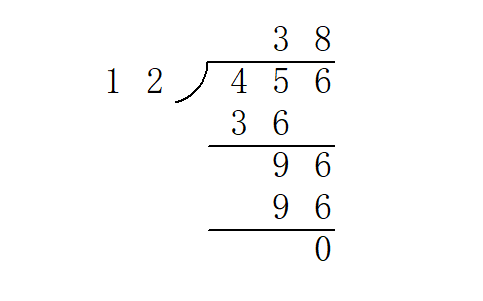
\includegraphics[width=4cm]{picture/Diversion vertical.png}
    \caption{高精度竖式除法}
\end{figure}

与高精度除以低精度类似,也是通过对被除数的每一位判断能否除以除数,将商留下,余数给下一位进行运算。但是这里不同的是,我们无法直接使用高精度除法。我们知道,除法是减法的累积,因此我们可以将除法转化为减法,当被除数的前i位再减除数就小于0时,跳到下一位。

竖式长除法实际上可以看作一个逐次减法的过程。例如下图中商数的十位的计算可以这样理解:将 $45$ 减去三次 $12$ 后变得小于 $12$,不能再减,故此位为 $3$。为了减少冗余运算,我们提前得到被除数的长度 $l_a$ 与除数的长度 $l_b$,从下标 $l_a - l_b$ 开始,从高位到低位来计算商。这和竖式除法时将第一次乘法的最高位与被除数最高位对齐的做法是一样的。



核心代码如下:

\begin{minted}
[
frame=lines,
framesep=2mm,
baselinestretch=1.2,
bgcolor=LightGray,
fontsize=\footnotesize,
linenos
]
{c}
int cmp(int A[], int B[]);
int greater_eq(int *a, int *b, int last_dg, int len);
void div(int A[], int B[]);

int main()
{
    if(!cmp(A, B))              // 如果A小于B,
    {
        printf("0\n%s\n", a);
    }
    else
    {
        div(A, B);
        for(int i = lenC - 1; i >= 0; i --) printf("%d",C[i]);
        printf("\n");
        for(int i = lenD - 1; i >= 0; i --) printf("%d",D[i]);
    }
    return 0;
}

int cmp(int A[], int B[])
{
    if(lenA != lenB)    return ((lenA > lenB) ? 1 : 0);
    for(int i = lenA - 1; i >= 0; i --)
    {
        if(A[i] != B[i])    return ((A[i] > B[i]) ? 1 : 0);
    }
    return 1;
}

// geq()用于判断被除数以下标digit为最低位,是否可以再减去除数而保持非负
// 此后对于商的每一位,不断调用 geq(),并在成立的时候用高精度减法从余数中减去除数
// 被除数 a 以下标 digit 为最低位,是否可以再减去除数b而保持非负
// len 是除数 b 的长度,避免反复计算
int geq(int *a, int *b, int digit, int len)
{
    // 有可能被除数剩余的部分比除数长,这个情况下最多多出 1 位,故如此判断即可
    if (a[digit + len] != 0) return 1;
    // 从高位到低位,逐位比较
    for(int i = len - 1; i >= 0; --i)
    {
        if(a[digit + i] > b[i]) return 1;
        if(a[digit + i] < b[i]) return 0;
    }
    // 相等的情形下也是可行的
    return 1;
}

void div(int A[], int B[])
{
    int la = lenA, lb = lenB, len = lenA + lenB + 1;
    for (la = len - 1; la > 0; -- la)
        if(A[la - 1] != 0)      break;
    for (lb = len - 1; lb > 0; -- lb)
        if(B[lb - 1] != 0)      break;
    // printf("%d %d %d\n", la, lb, len);
    if (lb == 0) 
    {
        // 除数不能为零
        printf("something wrong!\n");
        return;
    }
    // c 是商
    // d 是被除数的剩余部分,算法结束后自然成为余数
    for (int i = 0; i < la; ++ i) D[i] = A[i];
    for (int i = la - lb; i >= 0; -- i) 
    {
        // 计算商的第 i 位
        while(geq(D, B, i, lb))
        {
            // 若可以减,则做高精度减法
            for (int j = 0; j < lb; ++ j)
            {
                
                D[i + j] -= B[j];
                if(D[i + j] < 0) 
                {
                    D[i + j + 1] -= 1;
                    D[i + j] += 10;
                }
            }
            // 使商的这一位增加 1
            C[i] += 1;
            // 返回循环开头,重新检查
        }
    }
    lenC = lenA + lenB + 1;
    while (lenC > 1 && C[lenC - 1] == 0) lenC --;
    lenD = lenA + lenB + 1;
    while (lenD > 1 && D[lenD - 1] == 0) lenD --;
}
\end{minted}

\subsubsection{牛顿迭代法}

首先介绍牛顿迭代法,对于给定的一个函数$f(x)$,要求一个$f(X)=0$的根,可以选择一个临近这个根的点作为初始点$x_0$,然后求$f(x)$于$(x_0,f(x_0))$处切线与x轴的交点,此交点会更加接近根。

那么,迭代式如下:

\begin{equation*}
    x=x_0-\frac{f(x_0)}{f'(x_0)}
\end{equation*}

每次以$x$代$x_0$后继续迭代,一般最终$x_0$将趋于所求的根,并且在满足某些条件的情况下, 迭代是二阶收敛的, 也就是每迭代一次, 有效位数几乎增加一倍.这样达到n位精度只需要$O(logn)$的迭代次数。

假设已经实现了高精度实数运算,那么可以直接运用牛顿迭代法求解大整数的倒数。假如考虑方程$Ax-1=0$,那么迭代式为

\begin{equation*}
    x=x_0-\frac{A-1}{A} = \frac{1}{A}
\end{equation*}

很显然,这并没有解决问题,但如果考虑方程$\frac{1}{x} - A=0$,那么迭代式为

\begin{equation*}
    x = x_0 - \frac{\frac{1}{x_0}-A}{-\frac{1}{x_0^2}} = 2x_0-Ax_0^2
\end{equation*}

这里只有减法和乘法,因此估计一个较好的初值(可以取比$\frac{1}{A}$稍小的数),就能迭代得到$\frac{1}{A}$。得到$\frac{1}{A}$后,再乘$B$,取整后调整,即可得到$\lfloor \frac{B}{A} \rfloor$。

但是这里用到了不希望出现的高精度实数运算,那么需要寻找一种替代方式。

假如A有n位,那么我们希望求得$A'=\lfloor \frac{10^{2n}}{A} \rfloor$,然后计算$\lfloor \frac{BA'}{10^{2n}} \rfloor$ 后调整,即得$\lfloor \frac{B}{A} \rfloor$。不过这里面有个$A'$的舍入误差问题,为了保证最后调整次数是$O(1)$的,那么$A$相对$B$位数不能太少,假设$B$有$m$位,我们需要使得$m \leq 2n$,这样可以证明最后调整的时候,误差不超过10。这很简单,假如$m > 2n$,两者同时左移若干位即可。

下面的问题就是求解$\lfloor \frac{10^{2n}}{A} \rfloor$。设前一次迭代求解的是
$A^′_k = \lfloor \frac{10^{2k}} {A_k} \rfloor$ (其中$A_k$是$A$的前$k$位组成的数),那么这
一次的迭代式为

\begin{equation*}
    \frac{A'^{*}}{10^{2n}} = \frac{2A'_{k}}{\frac{10^{2k}}{10^{n-k}}}-A(\frac{A'_{k}}{\frac{10^{2k}}{10^{n-k}}})^2
\end{equation*}

也就是

\begin{equation*}
\begin{split}
    A'^* &= 2A'_k*10^{n-k}-\frac{AA_{k}^{'2}}{10^{2k}} \\
         &= 2A'_k*10^{n-k} - \lfloor \frac{AA_{k}^{'2}}{10^{2k}} \rfloor
\end{split}
\end{equation*}

求得$A'^{*}$当然还没完,这只是迭代的结果,并不是$\lfloor \frac{10^{2n}}{A} \rfloor$的准确值。误差分析表明,当$k > \frac{n}{2}$ 时,误差不超过100(可取$k = \lfloor \frac{(n + 2)}{2} \rfloor $),于是还要在求得余数$10^{2n} − AA′^∗$后对$A'^*$进行次数为$O(1) $的调整(为了降低常数, 可以二分误差)。这样就迭代地求解出了$\frac{10^{2n}}{A}$。边界条件是$n \leq 2$, 此时$A$在小整数范围内, 可以直接求解结果。

求解出$\frac{10^{2n}}{A}$后与$B$ 相乘, 再在计算余数后进行和上面类似的调整, 即可求解出$\lfloor 
\frac{B}{A}\rfloor$。

核心代码如下:

\begin{minted}
[
frame=lines,
framesep=2mm,
baselinestretch=1.2,
bgcolor=LightGray,
fontsize=\footnotesize,
linenos
]
{c}
poly operator / (poly a,poly b)
{
    if(a < b)   return poly{0};
    int n = a.size(), m = b.size();
    if(n > 2 * m)
    {
        a = a << (n - 2 * m);
        b = b << (n - 2 * m);
        n = a.size();
        m = b.size();
    }
    poly c = a * ~b >> 2 * m;
    if((c + poly{1}) * b <= a)
    {
        for(poly t = a - b * c; t >= b; t = t - b)
            c = c + poly{1};
    }
    else if(b * c > a)
    {
        for(poly t = b * c - a + b - poly{1}; t >= b; t = t - b) c = c - poly{1};
    }
    return c;
}
\end{minted}

\section{算法复杂性分析}

\begin{enumerate}
    \item 高精度加高精度:处理输入的字符串时时间复杂度为$O(n)$,加法过程为$O(n)$,因此高精度加高精度的时间复杂度为$O(n)$;
    \item 高精度减高精度:处理输入的字符串时时间复杂度为$O(n)$,比较大小后交换的时时间复杂度为$O(n)$,而做减法的时间复杂度为$O(n)$,因此高精度减高精度的时间复杂度为$O(n)$;
    \item 高精度乘低精度:高精度乘低精度的时间复杂度为$O(n)$;
    \item 高精度乘高精度:在做高精度与高精度的乘法的过程中,先对除数进行遍历,在每一位再对被除数进行遍历,因此高精度乘高精度的时间复杂度为$O(n^2)$;
    \item 快速傅里叶变换:$O(nlogn)$
    \item 快速数论变换:$O(nlogn)$
    \item 高精度除低精度:高精度除低精度只需要对被除数进行一次遍历,因此时间复杂度是$O(n)$;
    \item 高精度除高精度:高精度除高精度,首先对被除数进行遍历,再每次遍历的过程中进行复杂度为$O(n)$的高精度减法,因此高精度除高精度的时间复杂度为$O(n^2)$。
    \item 牛顿迭代法:$O(nlogn)$
\end{enumerate}

\section{测试}

对于附件中的Caculation程序,我们采用黑盒测试的方法,对其进行边界值测试与压力测试。

对于加法,我们测试了"123456789123456789 + 9786543214653864514658\\
4651",得到答案"97865432269995434270041440";当输入为“15321532447458\\745128465146512465164515486514865154865148651485148651487946516485\\13214651215648513546121564511356485154652514614851645 + 15321532447\\458745128465146512465164515486514865154865148651485148651487946516\\48513214651215648513546121564511356485154652514614851645”,输出"3064\\3064894917490256930293024930329030973029730309730297302970297302975\\89303297026429302431297027092243129022712970309305029229703290"。

对于减法,我们测试了"123456789 - 123456789",输出为"0";当输入为"12348651265 - 48551481548514865984",输出为"-48551481536166214719";输入为"4512451546654894589458945 - 123456",输出为"45124515466548\\94589335489"。

对于乘法,我们测试了"123 * 123",输出为"15129";输入为"99999999\\99999999999999999999999999999999999999999999999999999999999999999\\999999999999999999999999999 * 99999999999999999999999999999999999\\99999999999999999999999999999999999999999999999999999999999999999",输出为"999999999999999999999999999999999999999999999999999999999\\999999999999999999999999999999999999999999800000000000000000000\\00000000000000000000000000000000000000000000000000000000000000\\000000000000000001"。

对于除法,我们测试输入为"4551498589458 / 123"时,输出为"370040535\\72 102";输入为"0 / 123"时,输出为"0 0";输入为“123 / 0”时,输出为"something wrong!"。

此外,还在AcWing、洛谷、牛客等多个平台测试了代码,均正确。

\section{参考文献}
[1] 倪泽堃,理性愉悦:高精度数值计算,全国青少年信息学奥林匹克冬令营论文集,2012

[2] 张一飞,求n!的高精度算法,国际信息学奥林匹克竞赛中国国家集训队论文集,2001

[3] 月下桃子树,FWT(快速沃尔什变换)零基础详解(ACM/OI),https://zhuanlan.zhihu.com/p/41867199,2018

[4] 月下桃子树,FFT(快速傅里叶变换)0基础详解!附NTT(ACM/OI),https://zhuanlan.zhihu.com/p/40505277,2018

[5] 维基百科,https://en.wikipedia.org/wiki/Elementary\_function

\end{document}
